\documentclass[a4paper,14pt]{extreport}
    \usepackage[left=0.5cm,right=1.5cm,
    top=1.5cm,bottom=1.5cm,bindingoffset=0cm]{geometry}
    
\input{preambula.tex}
 




\begin{document}
\begin{center}\xmybox[green]{Мнацаканов Антон} $\quad$ \xmybox[red]{Вар. 5}\end{center}

%####################### 1 #######################
\begin{tcolorbox}[colback=blue!5!white!100,colframe=blue!75!black!90,width=19cm,righttitle=0.5cm, 
title= \center{\Large{\textbf{1}}}]
\begin{center}\bf{Дайте визначення поняття «інтерфейс».}\end{center}
\tcblower
Інтерфейс (англ. interface – засіб спряження, сполучення) це сукупність уніфікованих технічних і програмних засобів, необхідних для підключення зовнішніх пристроїв. Він забезпечує перетворення сигналів МП у сигнали, які сприймаються зовнішніми пристроями, і навпаки, підсилення сигналів та
являє собою апаратні засоби і набір програм передачі даних (уніфікований протокол обміну інформацією).\\

За способом передачі даних інтерфейси можна поділити на синхронні та асинхронні. При синхронному способі передавання даних робота передавального і приймального пристроїв синхронізується спеціальним синхронізуючим сигналом.\\ 

Крім того інтерфейси можна поділити на послідовні та паралельні. У послідовних інтерфейсах передавання (приймання) інформації здійснюється послідовно біт за бітом. При паралельному передаванні даних передається одночасно ціла група бітів. Як правило – це байт або слово.
\end{tcolorbox}


%####################### 2 #######################
\begin{tcolorbox}[colback=orange!5!white!100,colframe=orange!75!black!90,width=19cm,righttitle=0.5cm,
title= \center{\Large{\textbf{2}}}]
\begin{center}\bf{Що представляє собою ARM архітектура?}\end{center}
\tcblower
Архітектура ARM – це RISC архітектура на основі
ліцензованих 32-бітних і 64-бітних мікропроцесорних ядер розробки компанії ARM Limited.
\end{tcolorbox}


%####################### 3 #######################
\begin{tcolorbox}[colback=red!5!white!100,colframe=red!75!black!90,width=19cm,righttitle=0.5cm,
title= \center{\Large{\textbf{3}}}]
\begin{center}\bf{Перелічіть основні недоліки архітектури принстонського типу.}\end{center}
\tcblower
Зростаючі вимоги до продуктивності мікропроцесорних систем спричинили в останні роки перехід до архітектури з гарвардським типом доступу до пам'яті (з двома системними шинами), оскільки кожна пам'ять з'єднується з процесором окремої шиною, що
дозволяє одночасно з читанням або записуванням даних (при виконанні поточної команди) робити вибірку наступної команди. Завдяки такому розподілу потоків команд і даних та поєднанню операцій їх вибірки і виконання реалізується більш висока продуктивність, ніж при використанні архітектури
принстонського типу.
\end{tcolorbox}


%####################### 4 #######################
\begin{tcolorbox}[colback=green!5!white!100,colframe=green!75!black!90,width=19cm,righttitle=0.5cm,
title= \center{\Large{\textbf{4}}}]
\begin{center}\bf{Наведіть класифікацію арифметико-логічних пристроїв за способом дії
над операндами.}\end{center}
\tcblower
Всі виконувані в АЛП операції є логічними операціями (функціями),
які можна поділити на наступні групи:
\begin{itemize}
\item операції двійковій арифметики для чисел з фіксованою крапкою;
\item операції двійкової (або шістнадцяткової) арифметики для чисел з
плаваючою крапкою;
\item операції десяткової арифметики;
\item операції індексної арифметики (при модифікації адрес команд);
\item операції спеціальної арифметики;
\item операції над логічними кодами (логічні операції);
\item операції над алфавітно-цифровими полями.
\end{itemize}
\end{tcolorbox}


%####################### 5 #######################
\begin{tcolorbox}[colback=magenta!5!white!100,colframe=magenta!70!black!90,width=19cm,righttitle=0.5cm,
title= \center{\Large{\textbf{5}}}]
\begin{center}\bf{Опишіть схеми підключення послідовних периферійних інтерфейсів.}\end{center}
\tcblower
\center{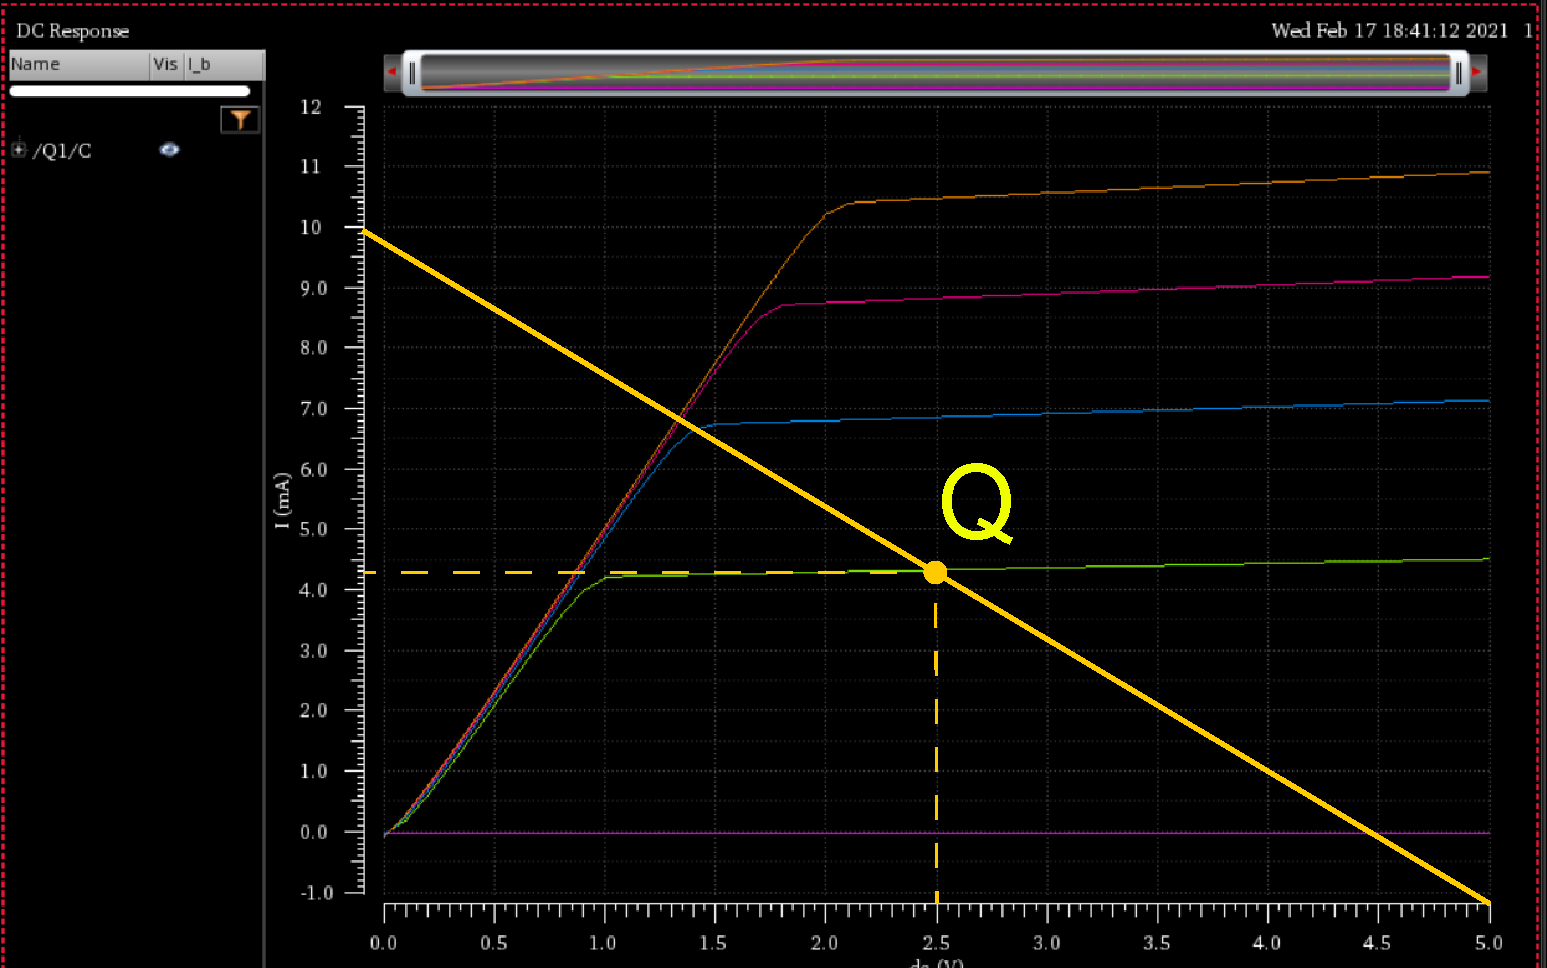
\includegraphics[width=0.7\linewidth]{1.png}}
\end{tcolorbox}



%####################### 6 #######################
\begin{tcolorbox}[colback=gray!5!white!100,colframe=gray!75!black!90,width=19cm,righttitle=0.5cm,
title= \center{\Large{\textbf{6}}}]
\begin{center}\bf{Що являє собою асинхронний послідовний інтерфейс RS-485?}\end{center}
\tcblower
Aсинхронний послідовний iнтерфейс RS-485 може існувати у двох варіантах: двопровідному і чотирипровідному. Двопровідний варіант використовується для напівдуплексної передачі, коли інформація може передаватися в обох напрямках, але в різний час. Для дуплексної передачі використовують чотири лінії зв'язку: за двома інформація передається в одному напрямку, за двома іншими – в зворотному. Недоліком чотирипровідної схеми є необхідність жорсткого визначення ведучого і ведених пристроїв на стадії проектування системи, в
той час як у двопровідній схемі будь-який пристрій може бути як в ролі ведучого, так і веденого. Перевагою чотирипровідної схеми є можливість одночасного передавання і приймання даних, що буває необхідно при реалізації деяких складних протоколів обміну.
\end{tcolorbox}

\end{document}